\subsection{Bilernes interaktion med andre mennesker}
I takt med at der kommer flere  selvkørende biler på vejene, er der kommet mere lys på de problemer som disse biler har når de har interaktioner med omgivelserne. En af de større udfordringer de har mødt, er selve trafikken og alt der hører med til denne. Bilens sensorer gør at den har en større årvågenhed end andre bilister, hvilket faktisk har vist sig at være et problem. Problemet er, at bilens opmærksomhed også sætter den i stor fare for at blive påkørt af en uopmærksom bilist som kommer kørende bagfra. Dette bekræfter Google selv i deres månedlige rapport fra august 2015\cite{GOOG_MONTHLY}. 

En anden udfordring de selvkørende biler har er, at de som de er nu kører ekstremt sikkert. I dette tilfælde skal ordet sikkert ikke tages på en god måde. Den selvkørende bil er bilen der virker som om den er lige lidt for langsom ud af lyskrydset, og som altid sikrer sig at den ikke overstiger fartgrænsen på nogen måde. Dette gør at den ellers travle trafik bliver sinket af de selvkørende biler som er på gaden. Denne form for kørsel ville i princippet ikke være et problem for bilen, men da der ikke er nogen mennesker der kører på helt samme måde, så skaber det som sagt nogen problemer. Et eksempel kunne være som vist her:

\begin{figure}[h!]
    \centering
    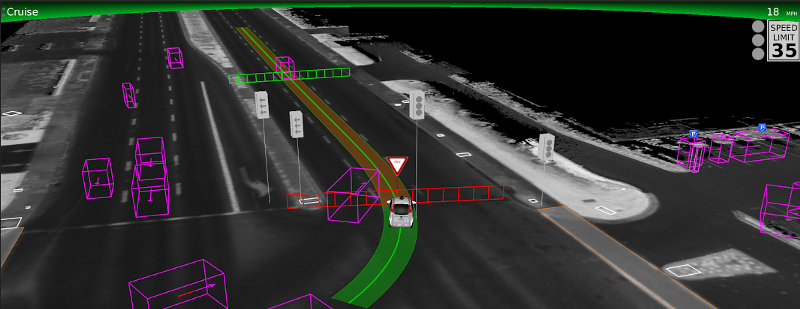
\includegraphics[width=0.8\textwidth]{images/google_vision.png}
    \caption{Bilens scan, der viser hvad der er i nærheden. Altså dens syn}
    \label{fig:car_vision}
\end{figure}

På billedet ses en situation som er et eksempel på dens kørsel. Her skal de pink kasser ses som andre køretøjer, og den grønne linje som bilens rute, og midt i selve billedet er bilen selv. Men situationen her er, at bilen på den venstre side af den selvkørende bil svinger lidt bredt, hvilket gør at den kommer ind i vores selvkørende bils bane. Så i stedet for at selv tage et lidt bredere sving, så kan det ses at den selvkørende bil bremser ned. Det kan ses ved det røde hegn foran bilen, som betyder at bilen bremser. 

En anden situation hvor sådan en bil fejlede i at reagere blev beskrevet af en cyklist i Austin, Texas, hvor han nemlig mødte en sådanne selvkørende bil i et kryds, mens han var på cykel. Cyklisten lavede så det man kalder en track-stand, men han lagde sig ind bag bilen. En track-stand er en teknik man bruger til at holde sig på cyklen når man kører rigtigt langsomt, hvor man så også bevæger styret på cyklen frem og tilbage for at holde balancen. Den selvkørende bil misforstod så denne track-stand for en cyklist der kom kørende bag den og stoppede. Så da bilen kunne se at cyklisten holdte stille kørte den så igen, hvorefter den så spottede igen fordi cyklisten bevægede styret fra den ene side til den anden. Dette gjorde at bilen stadig ikke var nået ud til midten af krydset efter hele 2 minutters kørsel\cite{VOX}. Det lyder måske ikke af meget, men det er sådanne problemer der er nødvendig at fokusere på at sikre der ikke sker på de forkerte tidspunkter, da begge hændelser ville have kunne føre til større ulykker, eller yderligere forsinkelser af trafikken. 